\section{Network Protocol and Architecture}

The \oscoin{} network protocol is a realization of the protocol semantics
described in \S~\ref{sec:protocol-semantics}, into the asynchronous network
model.

\subsection{Overview}

% TODO: Talk about BFT, 3f+1.
% TODO: Talk about the nodes/replicas.
% TODO: How does this work? Multi-chains etc, transactions, swaps, push/pull, git-remote-helper.
% TODO: How are patches constructed, how are repos constructed from patches.
% TODO: Staking and rate-limiting.
% TODO: Git remote-helper.
% TODO: Why patch-based systems are better.

The \oscoin{} network is composed of a set of nodes, or \emph{replicas}, which
execute a protocol $\mathcal{P}$. Together, these nodes form a \emph{Replicated
State Machine} with a set of states $\State^*$, a transition function $\delta$,
a starting state $\State_0$, a set of inputs $B_0 \dotso B_n$, and an empty set
of outputs $\varnothing$.

Participation in the network protocol is \emph{open}, which makes the replica
set \emph{dynamic}. To achieve consensus in the permissionless setting, we make
use of \emph{blockchains} as the underlying replicated data-structure, with the
assumption that a greater than $50\%$ majority of replicas are honest.
However, unlike other blockchain protocols, we describe a ``block-lattice''
design similar to~\cite{raiblocks}, with numerous advantages for our use case.

\subsubsection{Blockchain Architecture}

% TODO: Reference plasma?

\begin{description}
    \item[Sub-chain] hold source code in the form of repositories and
        patches.  They have members, issues and hold the balances to their
        native token.  Source chains function as a unit of governance.  In
        other words, organizations and communities are expected to operate
        under a single source chain.
    \item[Root chain] on the other hand functions as the canonical registry
        of all \emph{Source} chains. It holds the balances in oscoin.
\end{description}

\begin{figure}[htp]
    \documentclass[tikz]{standalone}

\usetikzlibrary{fit}
\usetikzlibrary{positioning}

\begin{document}
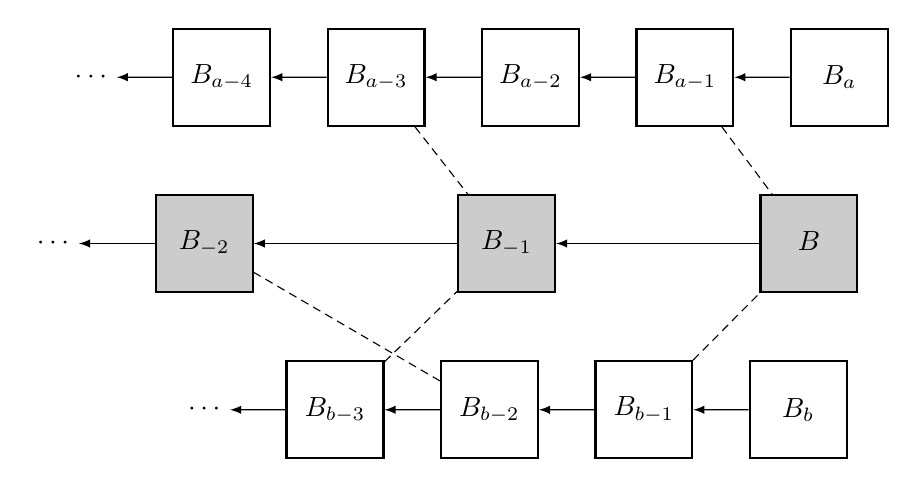
\begin{tikzpicture}[scale=0.96]
    \tikzstyle{root} = [draw=black, thick, fill=black!20, rectangle, minimum height=3.5em, minimum width=3.5em, node distance=3em];
    \tikzstyle{org-block} = [draw, thick, fill=white, rectangle, minimum height=3.5em, minimum width=3.5em, node distance=2em];
    \tikzstyle{link} = [-, thin, densely dashed];
    \tikzstyle{pointer} = [thin, -latex];

    \node (org-a-0) at (-2.5, 2.2)                {$\cdots$};
    \node[org-block] (org-a-1) [right=of org-a-0] {$B_{a-4}$}
        edge [pointer] (org-a-0.east);
    \node[org-block] (org-a-2)  [right=of org-a-1] {$B_{a-3}$}
        edge [pointer] (org-a-1.east);
    \node[org-block] (org-a-3)  [right=of org-a-2] {$B_{a-2}$}
        edge [pointer] (org-a-2.east);
    \node[org-block] (org-a-4)  [right=of org-a-3] {$B_{a-1}$}
        edge [pointer] (org-a-3.east);
    \node[org-block] (org-a-5)  [right=of org-a-4] {$B_{a}$}
        edge [pointer] (org-a-4.east);

    \node (root-0) at (-3, 0)        {$\cdots$};
    \node (root-1) at (-1, 0) [root] {$B_{\rootchain - 2}$}
        edge [pointer] (root-0.east);
    \node (root-2) at ( 3, 0) [root] {$B_{\rootchain - 1}$}
        edge [pointer] (root-1.east);
    \node (root-3) at ( 7, 0) [root] {$B_{\rootchain}$}
        edge [pointer] (root-2.east);

    \node (org-b-0) at (-1, -2.2) {$\cdots$};
    \node[org-block] (org-b-1) [right=of org-b-0] {$B_{b-3}$}
        edge [pointer] (org-b-0.east);
    \node[org-block] (org-b-2) [right=of org-b-1] {$B_{b-2}$}
        edge [pointer] (org-b-1.east);
    \node[org-block] (org-b-3) [right=of org-b-2] {$B_{b-1}$}
        edge [pointer] (org-b-2.east);
    \node[org-block] (org-b-4) [right=of org-b-3] {$B_{b}$}
        edge [pointer] (org-b-3.east);

    \draw [link] (org-a-2) -- (root-2);
    \draw [link] (org-a-4) -- (root-3);
    \draw [link] (org-b-2) -- (root-1);
    \draw [link] (org-b-1) -- (root-2);
    \draw [link] (org-b-3) -- (root-3);
\end{tikzpicture}
\end{document}

    \caption{Block-lattice design.}
\end{figure}

\bigskip

The advantages of this multi-chain design are numerous and are as follows.

\begin{enumerate}
    \item Scales horizontally with the number of communities.
    \item Clients with limited capacity can choose to support only certain
        communities at a lower cost, by syncing a subset of the chains.
    \item There is less centralization risk, since the sub-chains are more or
        less independent from the root chain.
    \item Latency on the sub-chains can be fairly low, since they don’t depend
        on a global consensus and don’t require a fixed block time.
    \item Security guarantees on the sub-chains can be relaxed compared to the
        root chain, since a compromised sub-chain cannot affect the root chain,
        and thus other sub-chains.
    \item Greater flexibility in chain governance and consensus, since
        sub-chains can choose a different trust model than the root chain.
    \item It's possible to mix permissioned and permissionless sub-chains,
        in the network \eg for hosting private repositories, since the
        interactions between chains are minimal and well specified.
    \item Allows forking at the community level, \eg when conflicts cannot be
        resolved through governance, it's possible to fork the whole source
        chain.
    \item The root chain becomes VCS agnostic.
\end{enumerate}

\subsection{Blocks, State and Transactions}

In \S~\ref{operations-and-state}, we saw that the protocol semantics could
be defined in terms of a global state $\State$ and a sequence of operations
$\op_1,\dots,\op_n$ applied to $\State$, forming a ledger $\Ledger$. When
describing the network architecture and protocol, a direct mapping between
these abstract objects and the components of the software architecture exist.

The state $\State$ is represented by a function $\State : K \to V$ which maps a
set of keys $K \in \mathbb{B}^{256}$ to a set of values $V \in \mathbb{B}^{*}$,
where $\mathbb{B}$ is the set of bytes, and $\mathbb{B}^n$ is the set of byte
strings of length $n$. The initial state $\State_0$ is called the
\emph{genesis} state. An operation $T$ is represented by a \emph{block}, and
the ledger $\Ledger$ by a \emph{blockchain}.

\subsubsection{State}

% TODO: $S[a]_n$: account $a$'s nonce.
% TODO: State transition function.
% TODO: Sender account has a nonce.

\subsubsection{Root Chain Transactions}

\begin{description}
    \item[Register] $\tx{register}{r_{org}}$: Registers a name on the root
        chain. Note that there is no `unregister' transaction, since
        withdrawing all existing deposits under the name and waiting a certain
        amount of blocks accomplishes this. (Figure~\ref{org-registration}.)
        \begin{figure}
            \documentclass[tikz]{standalone}

\begin{document}
\begin{tikzpicture}[scale=0.96]
    \tikzstyle{root} = [
        draw=black, thick, fill=black!20, rectangle, minimum height=4.5em, minimum width=4.5em, node distance=3em
    ];
    \tikzstyle{org-block} = [
        draw, thick, fill=white, rectangle, minimum height=3.5em, minimum width=3.5em, node distance=2em
    ];
    \tikzstyle{genesis-block} = [
        draw, fill=white, rectangle, minimum height=1em, minimum width=2em
    ];
    \tikzstyle{block-header} = [
        rectangle, minimum height=1em, minimum width=2em
    ];
    \tikzstyle{pointer} = [thin, -latex];

    \node (root-0) at (-3, 3) {$\cdots$};
    \node (root-1) at (-1, 3) [root] edge [pointer] (root-0.east);
    \node (root-2) at ( 3, 3) [root] edge [pointer] (root-1.east);
    \node (root-3) at ( 7, 3) [root] edge [pointer] (root-2.east);

    \node (root-1-header) [root-header, below=(2mm of root-1.north] {$B_^r{n-2}$};
    \node (root-2-header) [root-header, below=(2mm of root-2.north] {$B_^r{n-2}$};
    \node (root-3-header) [root-header, below=(2mm of root-3.north] {$B_^r{n-2}$};

    \node[genesis-block] (genesis-a) [above=(2.5mm of root-1.south)] {\small{$A_{0}$}};
    \node                (genesis-b) [above=(2.5mm of root-2.south)] {$\cdots$};
    \node                (genesis-c) [above=(2.5mm of root-3.south)] {$\cdots$};

    \node[org-block] (org-a-1) [below right=2em of root-1] {$B_^A{1}$};
    \node[org-block] (org-a-2) [right=of org-a-1] {$B_^A{2}$}
        edge [pointer] (org-a-1.east);
    \node[org-block] (org-a-3) [right=of org-a-2] {$B_^A{3}$}
        edge [pointer] (org-a-2.east);
    \node[org-block] (org-a-4) [right=of org-a-3] {$B_^A{4}$}
        edge [pointer] (org-a-3.east);
    \node[org-block] (org-a-5) [right=of org-a-4] {$B_^A{5}$}
        edge [pointer] (org-a-4.east);

    \draw [pointer, bend left=40] (org-a-1.west) to (genesis-a.south);
\end{tikzpicture}
\end{document}

            \caption{Org Registration. \label{org-registration}}
        \end{figure}
    \item[Update] $\tx{update}{u_{org}, u_{digest}, u_{height}, u_{P}}$. Commits
        a new source chain state to the root chain. The state digest and height
        are included in the transaction. This transaction is used by source
        chain validators to notify the root chain on progress.
    \item[Send] $\tx{send}{a_s, a_r, n}$. Send \oscoin{} to an address.
\end{description}

\subsubsection{Sub-Chain Transactions} \label{source-chain-transactions}

\begin{description}
    \item[Account] $\tx{account}{org, name, key}$. Registers a new user account
        with the given name and public key.
    \item[Patch] $\tx{patch}{org, repository, branch, p_P}$.  Add patches to a
        repo and branch. If the branch doesn’t exist, create it. If the
        repository doesn’t exist, create it. Since everything is managed with
        code, repository options and governance changes are also handled via
        this transaction.
    \item[Issue] $\tx{issue}{i_{org}, i_{repository}, i_{id}}$. Open an issue.
    \item[Amend] $\tx{amend}{i_{id}, i_{subject}, i_{body}, i_P}$.
        Update an issue's title, body or patch set.
    \item[Voice] $\tx{voice}{org, repository, issue, vote \in \{accept, reject\}}$
        Adds a voice to an issue. When a majority of voices have been heard in
        favor or against, the issue is accepted or rejected, respectively. This
        doesn’t mean the changes (if any) are merged immediately. In the case
        of a benevolent dictator, only their voice would be needed to resolve
        the issue.
    \item[Send] $\tx{send}{from, to, amount}$. Send org tokens to an address.
    \item[Set] $\tx{set}{org, key, value}$. Orgs wanting to store
        arbitrary metadata which is replicated and tamper-proof have the option
        of using this transaction. An empty value removes the key. This can be
        used as a package registry for example: \emph{Set(`bytestring',
        `https://hackage.haskell.org/package/bytestring')}
\end{description}

\subsubsection{Block}

A block $B$ in \oscoin{} consists of a block header $B_H$ and a sequence of
transactions $B_T$.

\begin{table}[hbtp]
    \begin{tabular}{l c p{7.5cm}}
        \toprule
        Field                  & Notation & Description \\
        \midrule
        \emph{Chain}           & $H_c$    & The name or identifier of the chain, \eg ``oscoin.'' \\
        \emph{Height}          & $H_n$    & The block height. \\
        \emph{ParentHash}      & $H_p$    & The \hash{} hash of the parent block header. \\
        \emph{TransactionRoot} & $H_{tr}$ & The root of the transaction hash tree. \\
        \emph{StateRoot}       & $H_{sr}$ & The \hash{} hash of the root of the state
                                            tree after all transactions in the block have
                                            been applied. \\
        \emph{Author}          & $H_a$    & The author of the block, and address to which
                                            all transaction fees collected in this block
                                            should be sent. \\
        \emph{Timestamp}       & $H_t$    & The local time of the author of this block at
                                            the time of authorship. \\
        \emph{ConsensusHash}   & $H_c$    & The \hash{} hash of the consensus parameters
                                            with which to validate the next block. \\
        \bottomrule
    \end{tabular}
    \medskip
    \caption{Block header fields \label{block-header-fields}}
\end{table}
